% \pagebreak[4]
% \hspace*{1cm}
% \pagebreak[4]
% \hspace*{1cm}
% \pagebreak[4]

\chapter{Existing solutions for the problem space}
\ifpdf
    \graphicspath{{Chapter1/Chapter1Figs/PNG/}{Chapter1/Chapter1Figs/PDF/}{Chapter1/Chapter1Figs/}}
\else
    \graphicspath{{Chapter1/Chapter1Figs/EPS/}{Chapter1/Chapter1Figs/}}
\fi

\nomenclature[zEDSR]{$EDSR$}{Enhanced Deep Super-Resolution Network}
\nomenclature[zPSNR]{$PSNR$}{Peak Signal-to-Noise Ratio}

\section{Enhanced Deep Super-Resolution Network (EDSR)}

\begin{figure}[!htbp]
  \begin{center}
    \leavevmode
    \ifpdf
      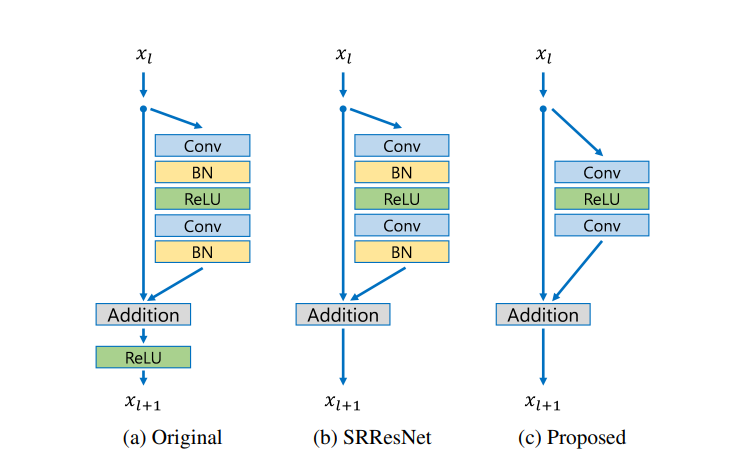
\includegraphics[height=3in]{Chapter1/Chapter1Figs/edsr.png}
    \else
      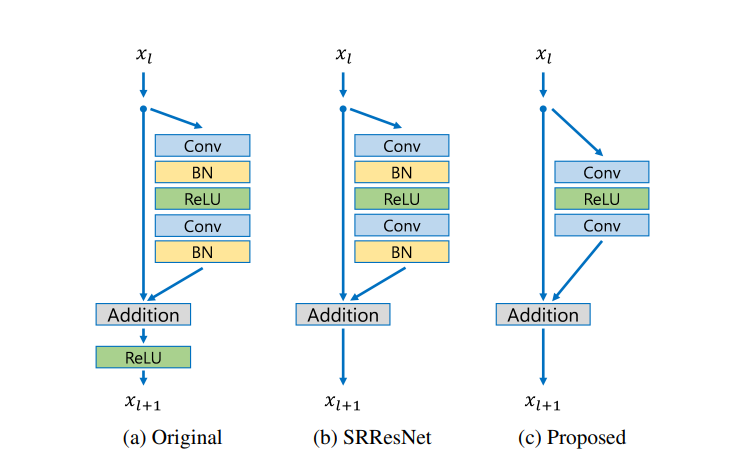
\includegraphics[bb = 92 86 545 742, height=6in]{Chapter1/Chapter1Figs/edsr.png}
    \fi
    \caption{ResNet vs SRResNet vs EDSR \cite{lim2017enhanced}}
    \label{EDSR Architecture}
  \end{center}
\end{figure}

The EDSR architecture \cite{lim2017enhanced} is based on the SRResNet architecture. It gives performance better than most state-of-the-art super-resolution models because it doesn't utilize the unnecessary modules present in conventional residual networks, and by increasing the model size.\\


An important feature of the EDSR network is that it can be used for higher magnifications such as 4X and 8X and has been used extensively for various kinds of super-resolution tasks. \\

Despite its large number of training parameters, EDSR is very simple to train and provides a very good PSNR for super-resolution, especially for medical imaging such as MRI which makes it a good baseline model for our work.\ref


\section{W-Net for MRI Reconstruction}

\begin{figure}[!htbp]
  \begin{center}
    \leavevmode
    \ifpdf
      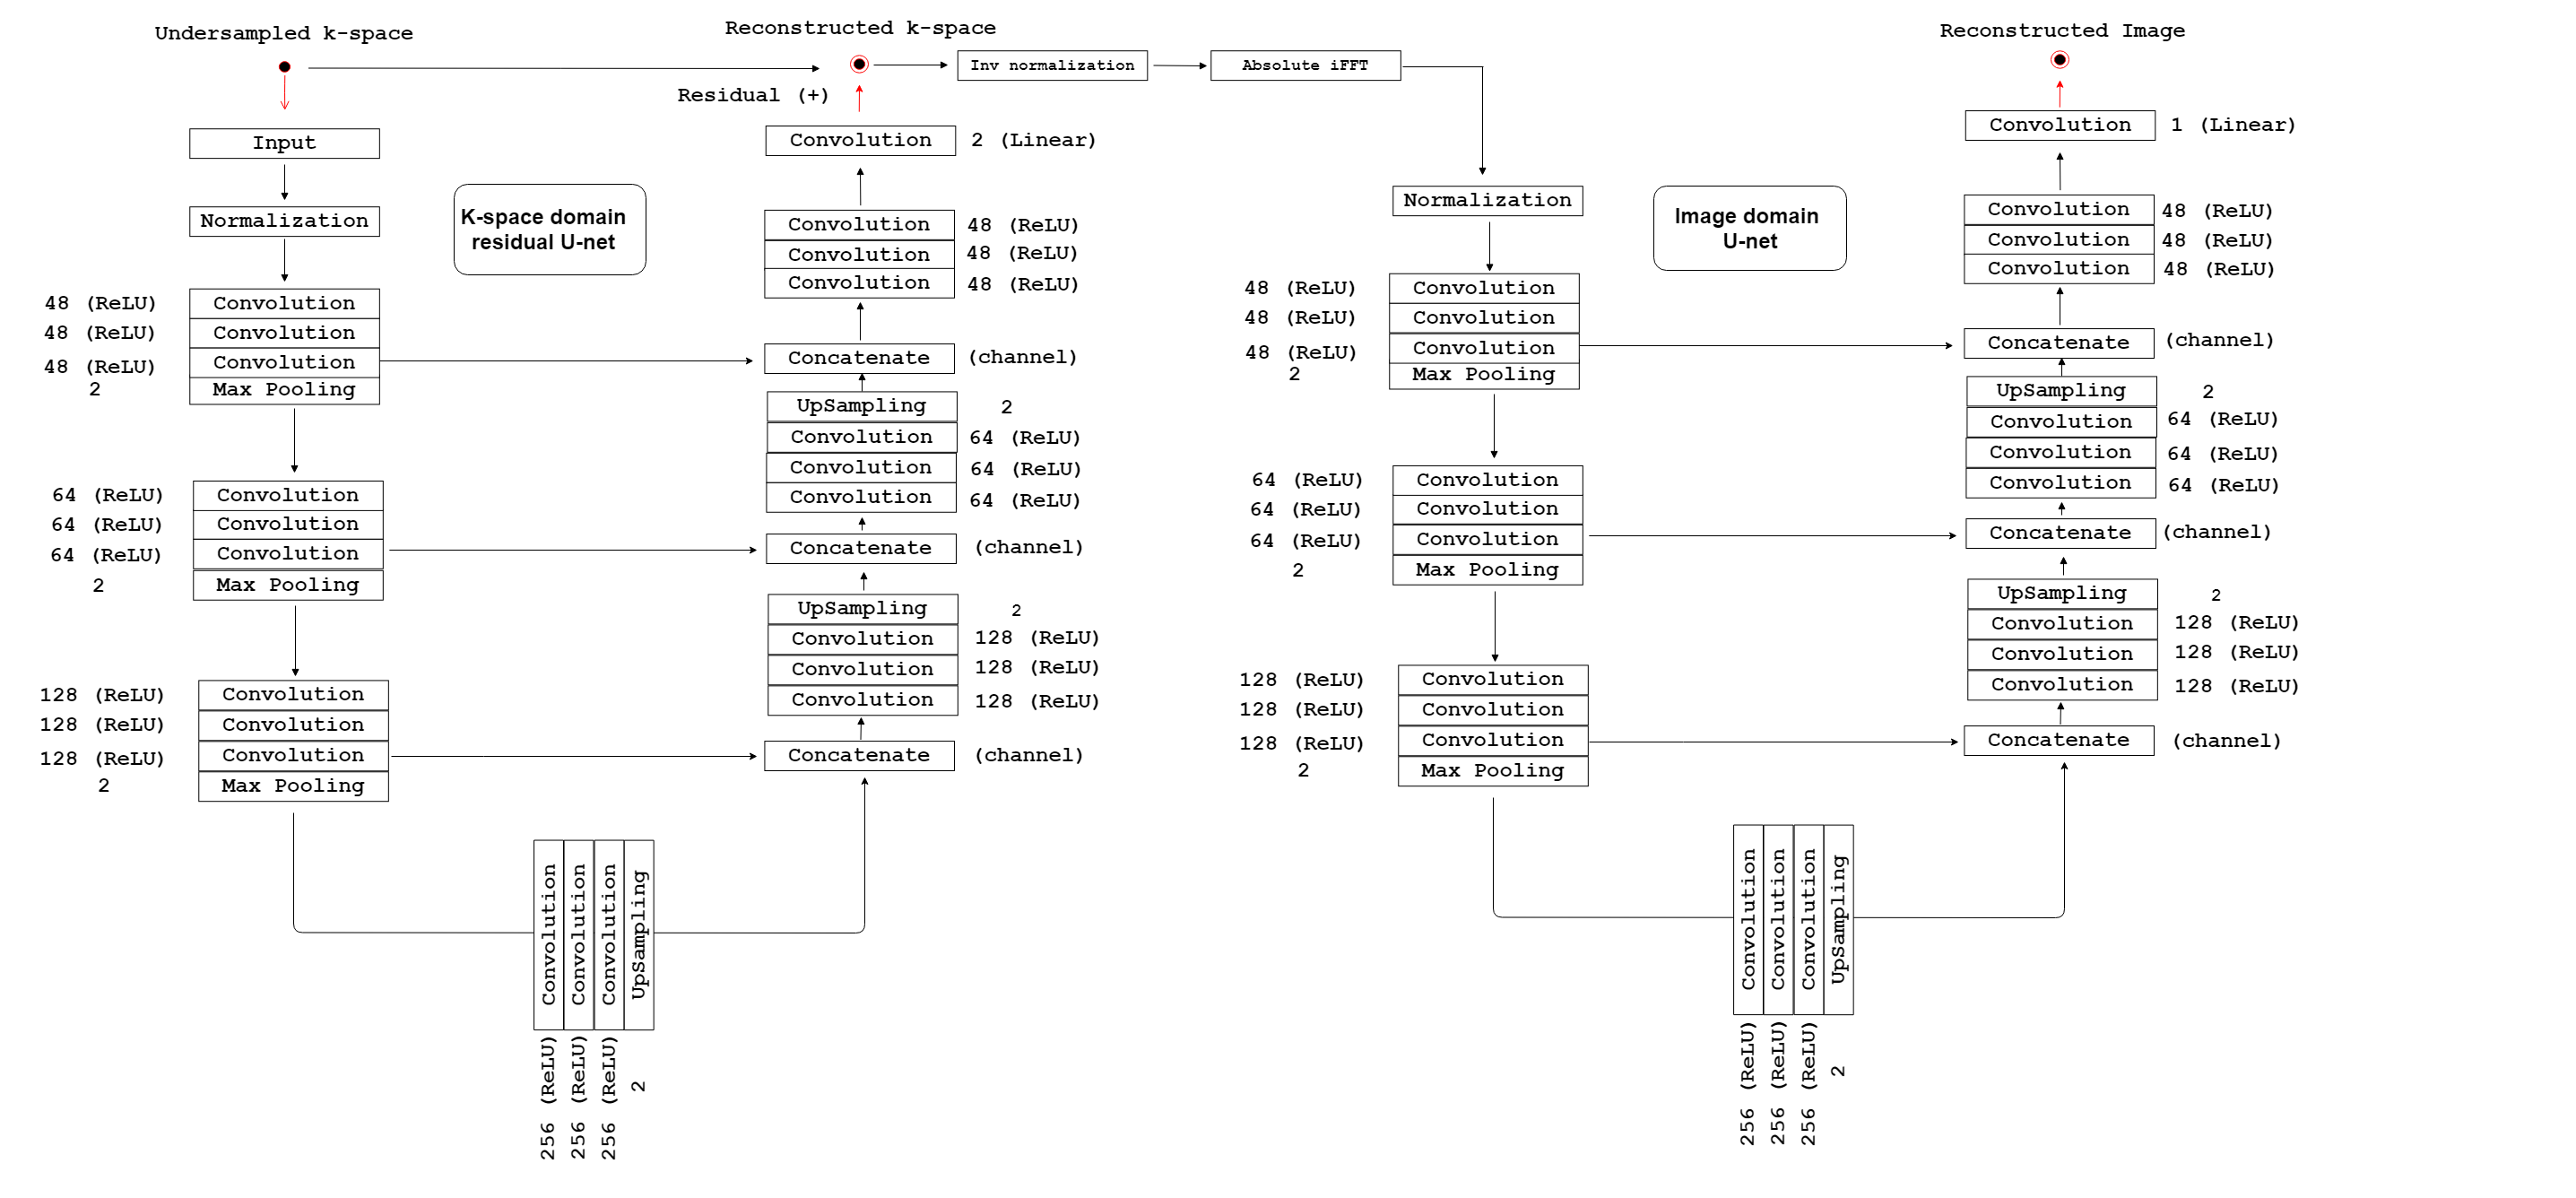
\includegraphics[height=3in]{Chapter1/Chapter1Figs/w-net.png}
    \else
      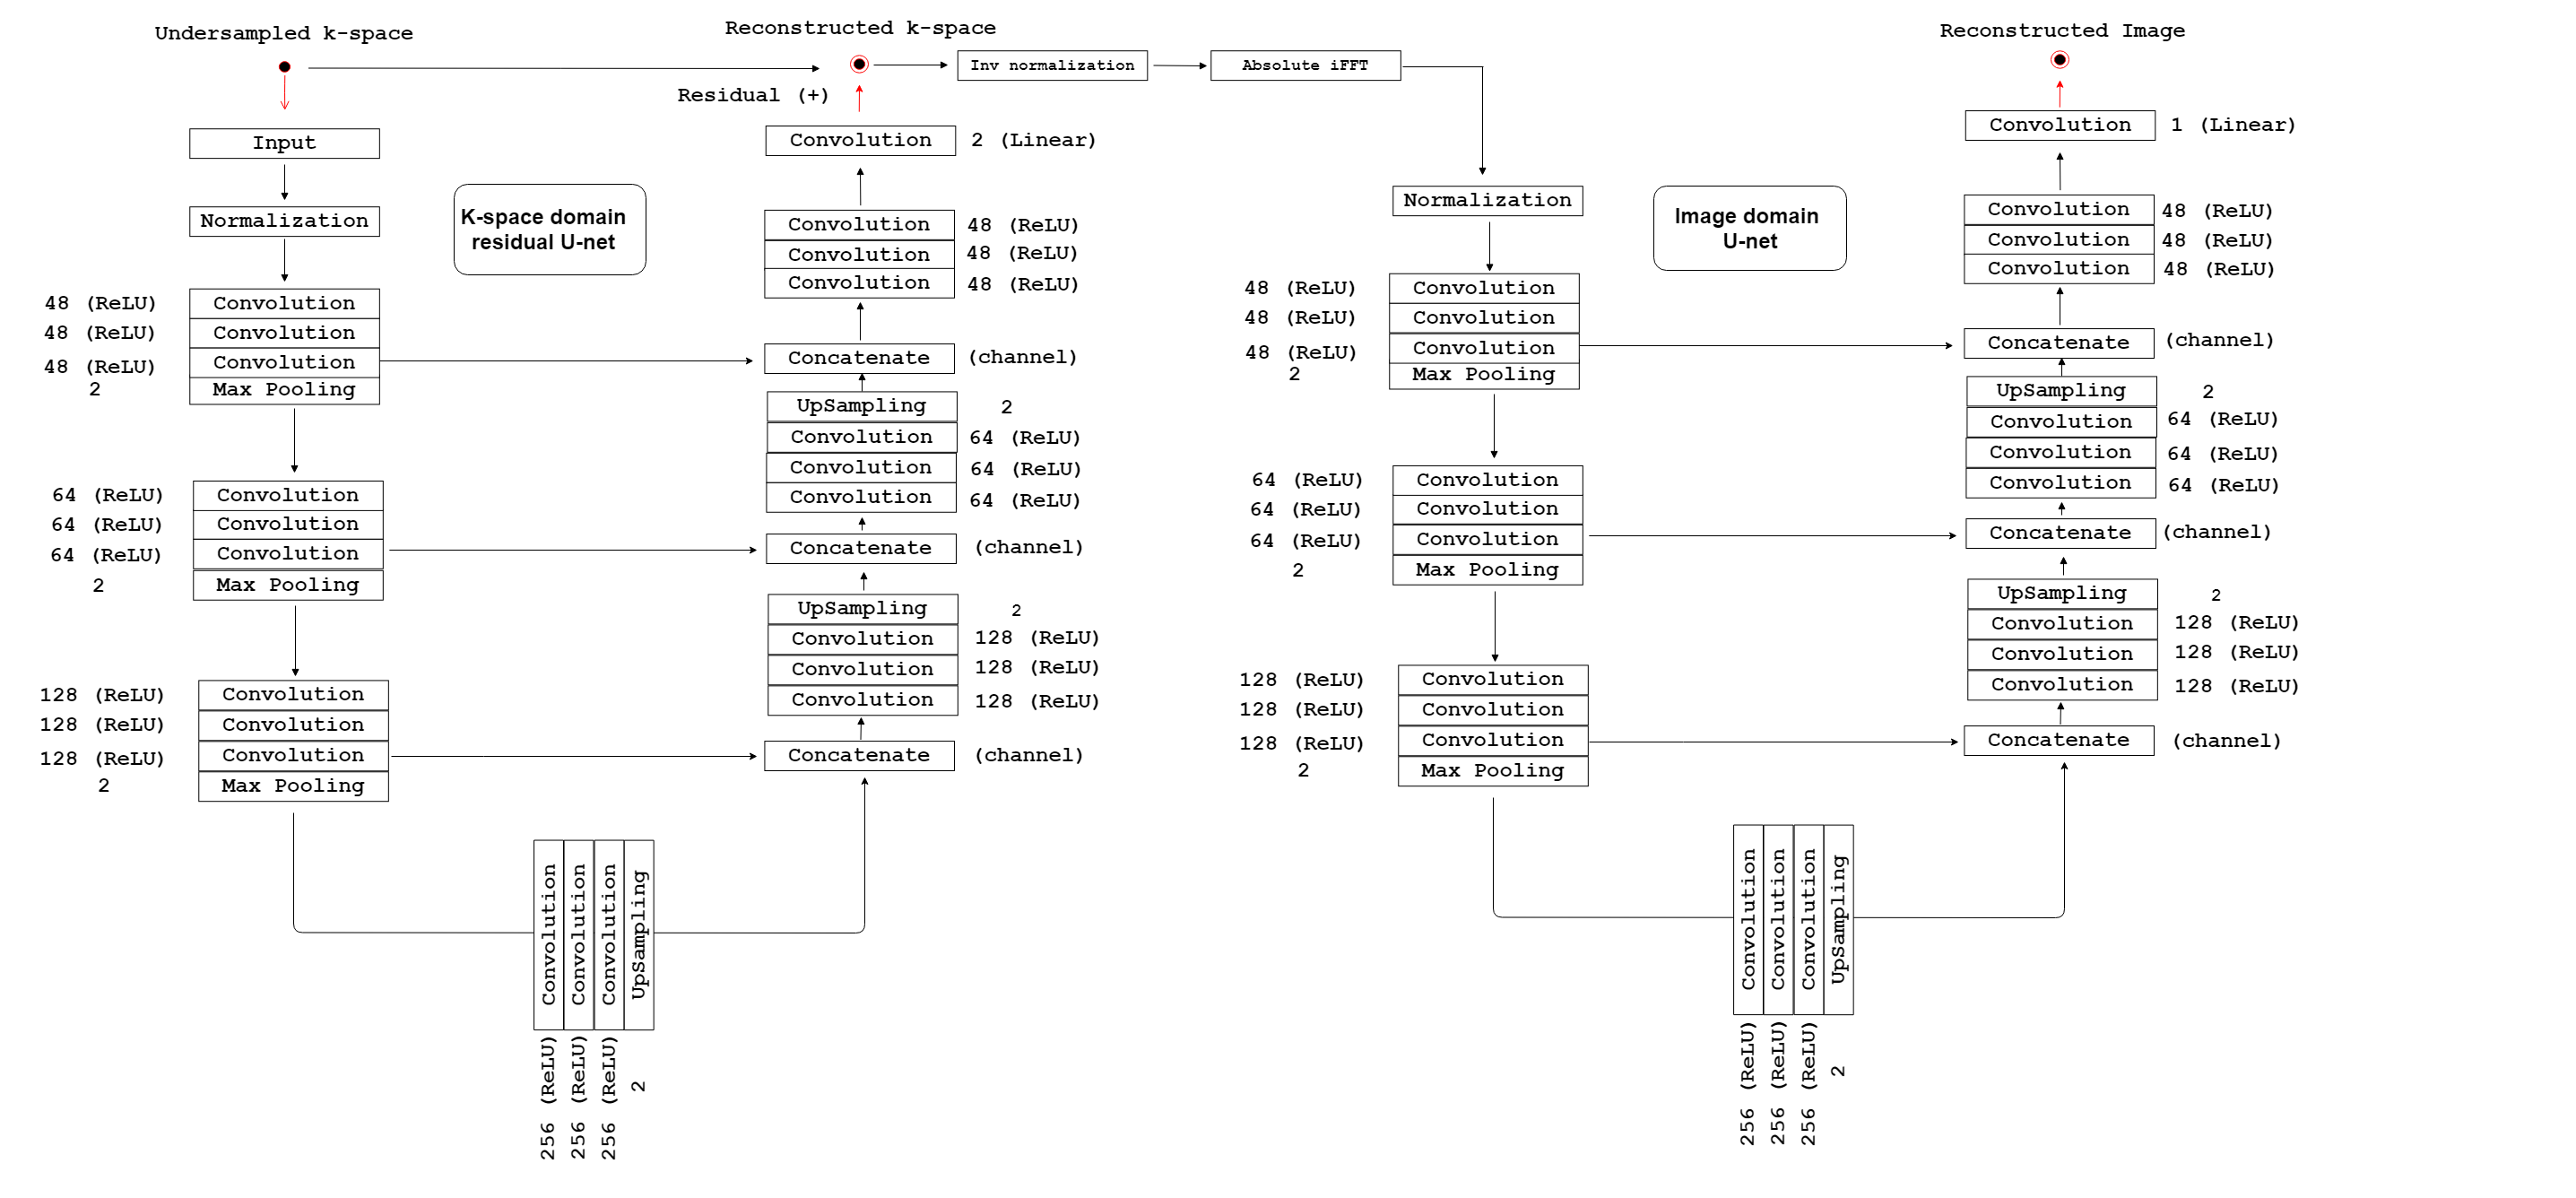
\includegraphics[bb = 92 86 545 742, height=6in]{Chapter1/Chapter1Figs/w-net.png}
    \fi
    \caption{W-Net architecture using two U-Nets \cite{8919674}}
    \label{W-Net model}
  \end{center}
\end{figure}

W-Net is an architecture that comprises two similar U-Nets and works both in the k-space (or frequency-domain) and the image (or spatial) domains. The model uses a complex-valued residual U-Net in the k-space domain, an iFFT operation, and a real-valued U-Net in the image domain (\cite{8919674}). This model is particularly suited to MR Images where there is an availability of raw k-space data to work with before it is converted into the image domain. The overall architecture can be seen in figure \ref{W-Net model} borrowed from \cite{xia2017wnet}.\\



This architecture displayed excellent results for reconstructing MR Images while utilizing lesser resources than other models such as GANs and Deep-Cascade networks. We aim to further enhance this model and tailor it further for MR Images.


\section{Super-Resolution via Repeated Refinements (SR3)}
\nomenclature[zSR3]{$SR3$}{Super-Resolution via Repeated Refinements}

Super-Resolution via Repeated Refinements (SR3) is a super-resolution diffusion model. Diffusion models have sprung up in recent years (\cite{saharia2021image}) as a model that provides accurate results, even more so than the popular Generative-Adversarial Networks (GANs \cite{goodfellow2014generative}) while being easier to train (\cite{dhariwal2021diffusion}).\\

Diffusion models have found their way into medical imaging and have become a popular option for the Super-Resolution of medical images. The SR3 model is trained by taking an image and adding noise to it progressively until only pure noise remains. The model learns to reverse this process so that it can create a high-resolution image from pure noise, iteratively, with guidance from the low-resolution image. Figure \ref{SR3-face} shows how SR3 works by removing noise to produce a high-resolution image, given the low-resolution image for reference (taken from \underline{\href{https://github.com/Janspiry/Image-Super-Resolution-via-Iterative-Refinement}{Janspiry's GitHub page}}).\\




Some popular implementations already exist and use well-known loss functions such as L1 and L2 for training to provide good results. This model showed very promising results, and due to it being a relatively very new model, it is under-researched. We aim to use this model for the super-resolution of MRIs.

\begin{figure}[!htbp]
  \begin{center}
    \leavevmode
    \ifpdf
      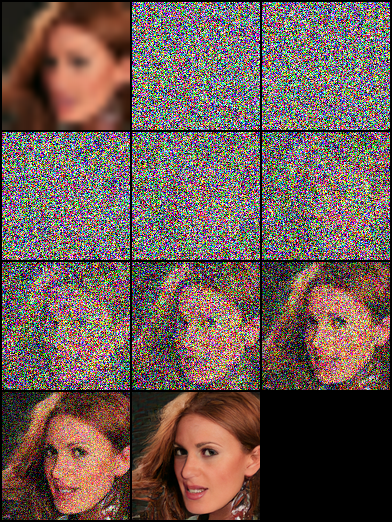
\includegraphics[height=4in]{Chapter1/Chapter1Figs/sr3.png}
    \else
      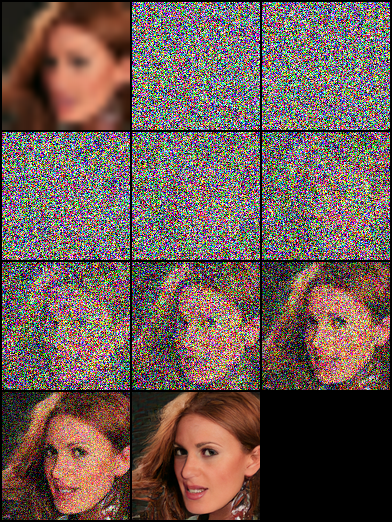
\includegraphics[bb = 92 86 545 742, height=6in]{Chapter1/Chapter1Figs/sr3.png}
    \fi
    \caption{Super-Resolution via Repeated Refinements on a face taken from \href{https://github.com/Janspiry/Image-Super-Resolution-via-Iterative-Refinement}{Janspiry's GitHub page}}
    \label{SR3-face}
  \end{center}
\end{figure}

% \nomenclature[zcif]{$CIF$}{Cauchy's Integral Formula}                                % first letter Z is for Acronyms 
% \nomenclature[aF]{$F$}{complex function}                                                   % first letter A is for Roman symbols
% \nomenclature[gp]{$\pi$}{ $\simeq 3.14\ldots$}                                             % first letter G is for Greek Symbols
% \nomenclature[gi]{$\iota$}{unit imaginary number $\sqrt{-1}$}                      % first letter G is for Greek Symbols
% \nomenclature[gg]{$\gamma$}{a simply closed curve on a complex plane}  % first letter G is for Greek Symbols
% \nomenclature[xi]{$\oint_\gamma$}{integration around a curve $\gamma$} % first letter X is for Other Symbols
% \nomenclature[rj]{$j$}{superscript index}                                                       % first letter R is for superscripts
% \nomenclature[s0]{$0$}{subscript index}                                                        % first letter S is for subscripts

% \section{Second Paragraph}
% and here I write more ...\cite{texbook}

% \subsection{sub first paragraph}
% ... and some more ...

% Now I would like to cite the following: \cite{latex} and \cite{texbook}
% and \cite{Rud73}.

% I would also like to include a picture ...

% \begin{figure}[!htbp]
%   \begin{center}
%     \leavevmode
%     \ifpdf
%       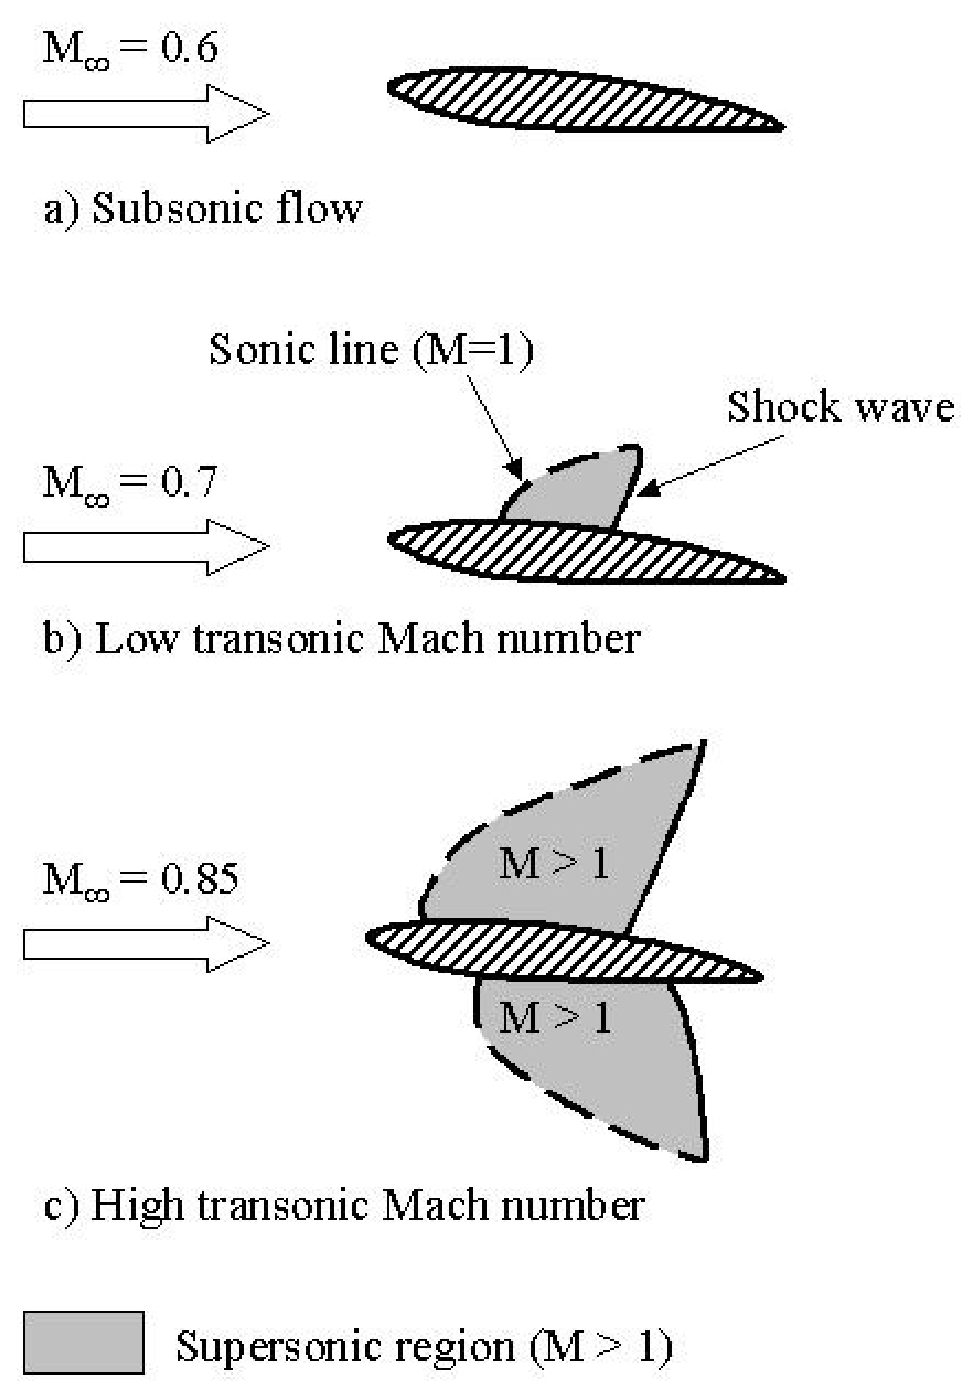
\includegraphics[height=6in]{aflow}
%     \else
%       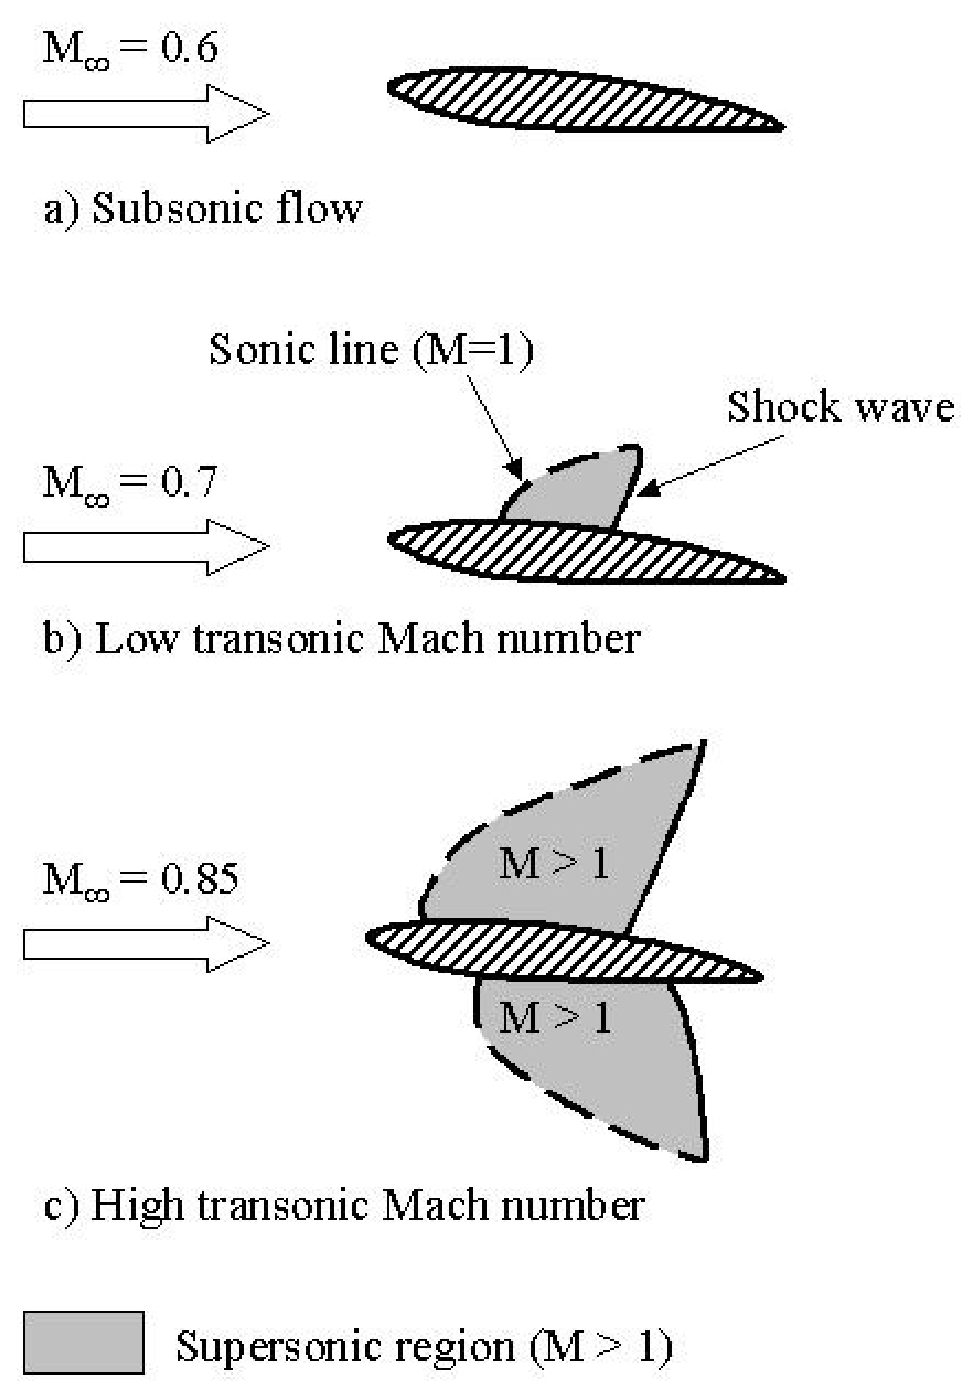
\includegraphics[bb = 92 86 545 742, height=6in]{aflow}
%     \fi
%     \caption{Airfoil Picture}
%     \label{FigAir}
%   \end{center}
% \end{figure}

% % above code has been macro-fied in Classes/MacroFile.tex file
% %\InsertFig{\IncludeGraphicsH{aflow}{6in}{92 86 545 742}}{Airfoil Picture}{FigAir}

% So as we have now labelled it we can reference it, like so (\ref{FigAir}) and it
% is on Page \pageref{FigAir}. And as we can see, it is a very nice picture and we
% can talk about it all we want and when we are tired we can move on to the next
% chapter ...

% I would also like to add an extra bookmark in acroread like so ...
% \ifpdf
%   \pdfbookmark[2]{bookmark text is here}{And this is what I want bookmarked}
% \fi
% ------------------------------------------------------------------------


%%% Local Variables: 
%%% mode: latex
%%% TeX-master: "../thesis"
%%% End: 
